\section{Database}

The database was hosted on Google Cloud Firestore, which provides a NoSQL JSON-compatible document-based database system. This significantly affected the database design of the project, as it introduced constraints on available database lookup and filtering features.

\subsection{Database Design}

The database design itself was created iteratively in collaboration with the entire backend team, based on the requirements of each individual search component. For convenience, the design diagram was compiled into an image file, accessible to the team through the GitHub.

Essentially, each backend component had its own collection, storing documents following a format described in the diagram. Each added page was given a unique ID number, which was used as the document name for the component collections. These collections were then unified by the 'pages' collection, storing metadata about each indexed page (including the page title, URL and ID). In addition, there was a collection with a document containing the last known page ID for when new pages were added, as well as a collection containing the vocabulary set used by the meanings component.

The database design diagram was created using the tool "draw.io". It highlights each collection, the document structure for each, as well as expected data types of each element. It can be seen on figure \ref{fig:db_design}.

For ease of use, within the backend, a set of wrapper functions was developed in a file called 'dbUtil.js'.

\newpage
\begin{figure}[!hb]
    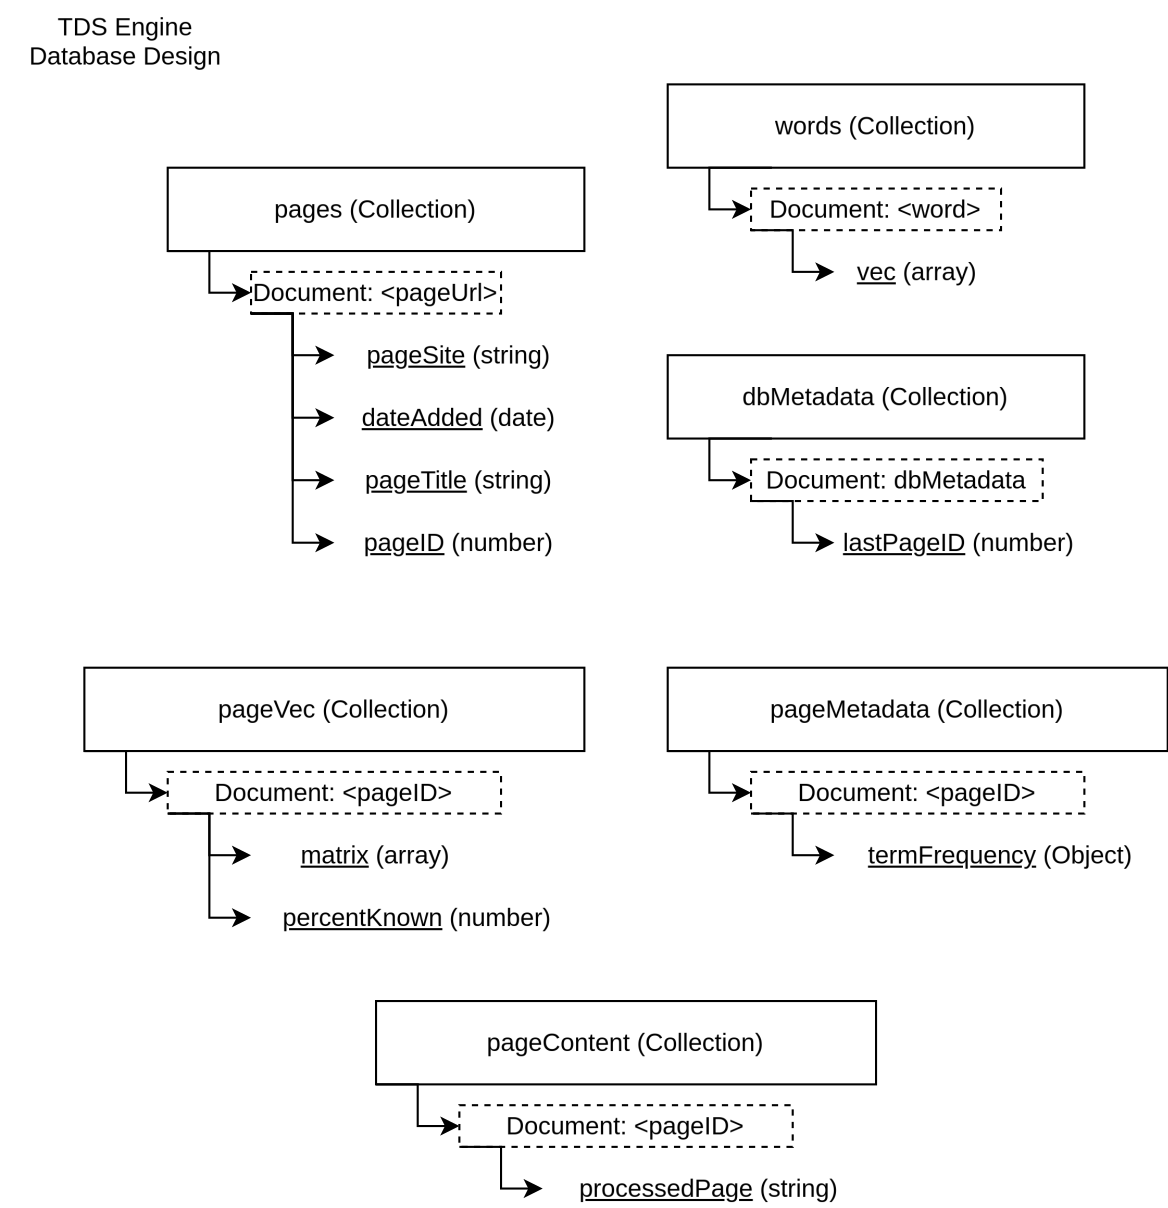
\includegraphics[width=\textwidth,keepaspectratio]{db_design.png}\\
    \caption{Database Design Diagram}
    \label{fig:db_design}
\end{figure}
\newpage


\subsection{Uploading Vocabulary}
To use the meanings search, a lookup table of word embedddings must be created in the database which can be accessed by functions. This is the collection titled Words. \\
Due to time constraints, a pre-trained list of word embeddings was downloaded in form of a txt file. This file contained 400k 50-dimensional word embeddings and their respective words. 
This file was then read into a function which turned them into an array of vectors indexed by the words. Then many downloaded html pages of technical documentation (mainly manual pages, but also documentation on different languages and general articles about computer science) were passed into the programme. These were processed by the text processing functions to be used on all pages added to the database to remove stopwords and punctuation. Then each file was read through and if a word in the file was found in the array of word embeddings, it was added to the database. Thus the 400k vectors were reduced to just over 5000 words which are commonly found in the sort of texts to be searched by the engine.    

\subsection{WordPages - a retired feature}
To make the search function more efficient a plan was conceived to filter pages based on words that appeared frequently in them. \\
When adding pages, each word is checked for its frequency and if it's above a certain threshold, the page ID is entered into a firestore document of that word. \\
When searching, only the pages found in the wordPages entries for each word in the query are checked. This was meant to make search more efficient, since it reduced the number of pages being checked for each query. \\
However, the wordPages feature was retired after it was found to result in less accurate searches. With more time, it could potentially be fine-tuned into creating a more accurate and efficient search engine. 
